% % % % % % % % % % % % % % % % % % % % % % % % % % % % % % % % % % % % % % % % %
\section{Die Bibliothek free-theorems}
% % % % % % % % % % % % % % % % % % % % % % % % % % % % % % % % % % % % % % % % %

\label{sec:free-theorems}

Die Generierung freier Theoreme ist geradlinig und unkompliziert. Gerade deshalb ist es jedoch mühselig, diese Arbeit jedes
Mal per Hand durchzuführen, da ja immer die gleichen Schritte durchgeführt werden. Von daher ist es wünschenswert, diesen
Prozess zu automatisieren, und genau das macht die Bibliothek \textit{free-theorems} \cite{freetheorems}. Diese Bibliothek
beinhaltet die Werkzeuge, die nötig sind, um freie Theoreme aus Haskell-Programmcode zu generieren.

In diesem Kapitel wird näher darauf eingegangen, welche Werkzeuge dies sind und wie sie zusammenspielen. Es wird erläutert,
welche Schritte notwendig sind, um aus Quellcode eine Formel herzuleiten, die das entsprechende freie Theorem darstellt.
Abgeschlossen wird diese Übersicht dann mit einem kleinen Beispiel, anhand dessen das Zusammenspiel der einzelnen
Datentypen zwischen den verschiedenen Funktionen veranschaulicht wird.

%In \cite{freetheorems} wird eine Implementierung vorgestellt, die die automatisierte Generierung von freien Theoremen aus
%Haskell-Code ermöglicht und die Grundlage darstellt, auf die die vorliegende Arbeit aufbaut.
%Sie erlaubt das Parsen von Haskell-Code, das Herausfiltern der entsprechenden Definitionen und deren relationale
%Interpretation, um schließlich die freien Theoreme zu erzeugen.
%Beigefügte Pretty printing Funktionen für Haskell-Syntax und Theoreme vereinfachen schließlich deren Darstellung.

%Im folgenden Abschnitt wird erläutert, wie diese Bibliothek grundlegend aufgebaut ist, wobei auf jeden einzelnen Schritt genauer
%eingegangen wird.


% - - - - - - - - - - - - - - - - - - - - - - - - - - - - - - - - - - - - - - - - - - - - - - - - - - - - - - - - - - - - - - - - - - - - - - - - - - - - - -
\subsection{Aufbau}
% - - - - - - - - - - - - - - - - - - - - - - - - - - - - - - - - - - - - - - - - - - - - - - - - - - - - - - - - - - - - - - - - - - - - - - - - - - - - - -

Die Bibliothek lässt sich grundsätzlich in drei Teile untergliedern: Frontend, Core und Pretty Printer \cite{freetheorems}, wobei
die Bibliothek auch in dieser Reihenfolge durchlaufen wird, zu sehen in Abbildung \ref{fig:overview}.

\begin{figure}[ht]
\centering
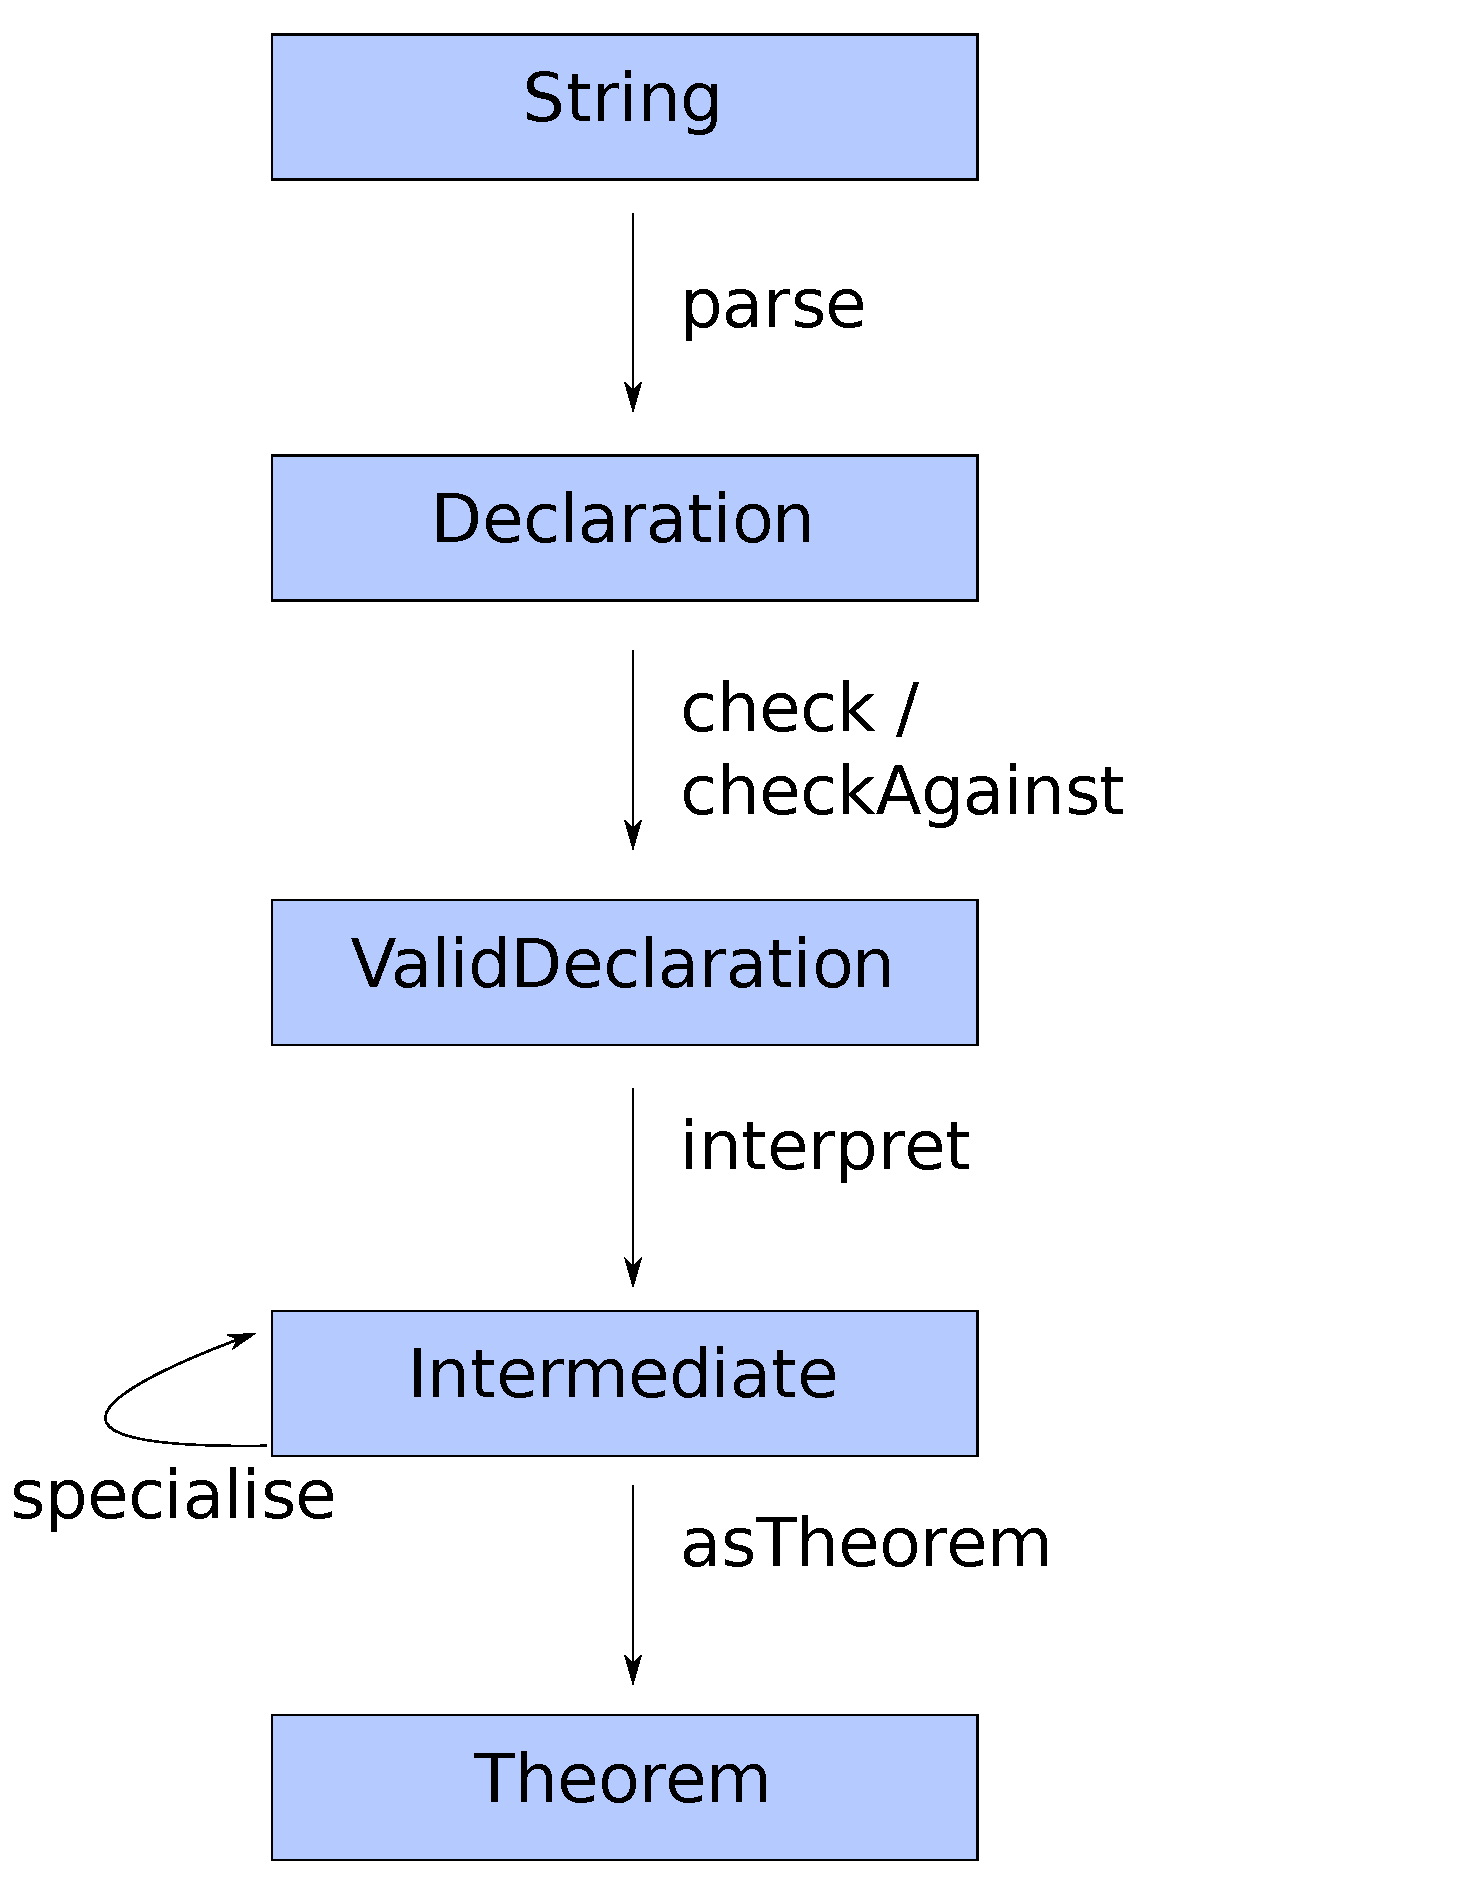
\includegraphics[height=300px]{overview-free-theorems}
\caption{Überblick über die Bibliothek free-theorems}
\label{fig:overview}
\end{figure}

Das Frontend ist der Teil, der den Haskell-Code entgegennimmt. Hier wird zunächst der Programmcode geparst und in einen
abstrakten Syntaxbaum übersetzt. Außerdem ist das Frontend dafür zuständig, Fehlerprüfungen durchzuführen und
ungültige Definitionen herauszufiltern, bevor der Syntaxbaum dann weiter an den Core gegeben wird.

%Zunächst werden im Frontend Parser bereitgestellt, um den Haskellcode aus einer Zeichenkette in eine passende Syntaxbaumstruktur umzuwandeln. Mithilfe einer check-Funktion
%wird diese Datenstruktur auf Gültigkeit überprüft, insbesondere in Bezug auf spezielle Anforderungen, die an die Definitionen gestellt wird, um Theoreme zu generieren.

Im Core findet die eigentliche Arbeit statt: Hier wird der Syntaxbaum in die entsprechende Relationaldarstellung
überführt und in eine Zwischendarstellung abgelegt, \texttt{Intermediate} genannt. Im nächsten Schritt wird diese
Relationaldarstellung dann Schritt für Schritt abgerollt und in eine Formel überführt. Diese Formel wird schließlich zurückgegeben.

Um diese Formel darzustellen, werden dann im Pretty Printer Teil entsprechende Funktionen bereitgestellt, die in der Lage
sind, den Formel-Datentypen in Zeichenketten umzuwandeln.

%\texttt{interpret} ist dann schließlich die Funktion, die eine Signatur in Bezug auf die anderen Deklarationen in eine Zwischendarstellung \texttt{Intermediate} überträgt. Die
%Funktion \texttt{asTheorem} entfaltet diese Darstellung \todo{``entfaltet''?} schließlich und überträgt sie in den Datentyp \texttt{Theorem}.


% - - - - - - - - - - - - - - - - - - - - - - - - - - - - - - - - - - - - - - - - - - - - - - - - - - - - - - - - - - - - - - - - - - - - - - - - - - - - - -
\subsection{Parser}
% - - - - - - - - - - - - - - - - - - - - - - - - - - - - - - - - - - - - - - - - - - - - - - - - - - - - - - - - - - - - - - - - - - - - - - - - - - - - - -

Um zu einer in Haskell geschriebenen Funktionssignatur irgendetwas zu generieren, muss zunächst eins getan werden: Aus dem
Programmcode muss die notwendige Information herausgezogen werden, der Haskell-Code muss geparst werden.
\textit{free-theorems} erfindet hier das Rad nicht neu sondern setzt auf einen Haskell-Parser, der mit \texttt{haskell-src-exts}
bereits als Paket verfügbar ist \cite{haskellsrcexts} \todo{cite} (bzw. \texttt{haskell-src} als Version, die keine
Spracherweiterungen unterstützt).

Dieses Paket bietet einen Parser für den kompletten Sprachumfang von Haskell inklusive aller Spracherweiterungen, die GHC
unterstüzt \cite{xyz} \todo{cite}. Der Parser liefert eine eigene Datenstruktur für einen abstrakten Syntaxbaum, aber der
enorme Sprachumfang hat natürlich zur Folge, dass dieser Syntaxbaum sehr komplex werden kann. Nun werden aber gar nicht
sämtliche syntaktischen Möglichkeiten der Sprache benötigt, ganz im Gegenteil: Für die Generierung freier Theoreme spielen
hauptsächlich Typsignaturen eine Rolle. Die Implementierungen, die in einem typischen Programm den Großteil des Programms
ausmachen, können getrost vernachlässigt werden.

Aus diesem Grund führt \textit{free-theorems} eine eigene Syntaxbaum-Datenstruktur ein und überführt den Syntaxbaum,
der von \texttt{haskell-src-exts} generiert wird, in eine vereinfachte Darstellung, genannt \texttt{BasicSyntax}.

%Neben dem Haskell 98 Parser, der keine \todo{Keine?} Spracherweiterungen zulässt, ist auch der Hsx Compiler gegeben, der die
%komplette Sprache mitsamt Spracherweiterungen umsetzt. Hier ist anzumerken, dass das Paket free-theorems in seiner aktuellen Form
%nicht mit dem aktuellen Haskell-Compiler kompatibel war und einige Anpassungen gemacht werden mussten. \todo{Evtl im Anhang Näheres?}
%Intern nutzt free-theorems hier die Pakete \texttt{Language.Haskell.Parser} bzw. \texttt{Language.Haskell.Exts.Parser}, die an sich bereits voll funktionstüchtige Parser liefern.

%Allerdings ist der komplette Sprachumfang sehr komplex und ein Arbeiten mit den Datenstrukturen, die von diesen genutzten Parsern generiert werden,
%wird unnötig erschwert. Aus diesem Grund transformiert free-theorems diese Datenstruktur in eine eigene, vereinfachte Struktur namens BasicSyntax. In dieser Struktur
%werden lediglich Typsignaturen festgehalten, Implementierungen werden vollkommen ignoriert, da sie für die Theoremgenerierung keine Rolle spielen.


\subsubsection*{BasicSyntax}
% `````````````````````

\label{sec:basic-syntax}

Ein paar kleine Beispiele sollen ein Gefühl dafür vermitteln, wie der \texttt{BasicSyntax}-Datentyp aussieht. Dabei ist jeweils
eine Funktionssignatur gegeben und dahinter die Haskell-Darstellung des resultierenden BasicSyntax-Ausdrucks.

\begin{listing}[ht]
%\inputminted[tabsize=2]{haskell}{ast.hs}
\begin{minted}{haskell}
test :: a -> b

[TypeSig
   (Signature {
      signatureName = Ident "test" ,
      signatureType =
         TypeFun
            (TypeVar (TV (Ident "a")))
            (TypeVar (TV (Ident "b")))
   )
]

\end{minted}
\caption{Beispiel}
\label{lst:ast}
\end{listing}

Listing \ref{lst:ast} zeigt die Datenstruktur am Beispiel \texttt{test :: [a] $\rightarrow$ [a]}. Die \texttt{parse}-Funktion des Parser-Moduls von \textit{free-theorems} liefert eine Liste sämtlicher relevanter Definitionen als \texttt{BasicSyntax} zurück.
In diesem Beispiel ist nur eine Typsignatur gegeben, \texttt{parse} gibt also eine einelementige Liste zurück, bestehend aus
genau einem Konstruktor \texttt{TypeSig}, der eine Typsignatur repräsentiert. Der Datentyp erwartet einen
\texttt{Signature}-Konstruktor, der as dem Namen der Signatur sowie einem Typausdruck besteht.

In diesem Fall ist der Typausdruck eine Funktion zwischen zwei Typvariablen, der Konstrktor \texttt{TypeFun} wird also
auf zwei \texttt{TypeVar}-Konstruktoren angewandt, die jeweils die Variablennamen beinhalten.

Da man freie Theoreme aus den Typsignaturen von Funktionen herleitet, könnte man sich überlegen, dass man auf alles andere
als Typsignaturen verzichten kann und der Rest des Programms irrelevant ist. Während Funktionsrümpfe, also die Implementierungen
der Funktionen, tatsächlich keinerlei Relevanz für freie Theoreme haben, gibt es dennoch Deklarationen neben Typsignaturen, an
denen man ebenfalls interessiert ist.

%Während dies für Implementierungen der Funktionen,
%also die jeweiligen Funktionsrümpfe, zutrifft, gibt es dennoch andere Deklarationen, an denen man ebenfalls interessiert ist.

Problematisch wird es nämlich sonst, wenn der Anwender der Bibliothek in seinem Programm eigene Datentypen deklariert und
diese in der zu Funktionssignatur verwendet. Neben Funktionssignaturen werden also zusätzlich auch Datentypdeklarationen
benötigt.
%Man bekommt nämlich genau dann ein Problem, wenn der Entwickler im Programm eigene Datentypen deklariert und diese in
%den Funktionssignaturen verwendet. Neben Funktionssignaturen werden also zusätzlich auch Datentypdeklarationen benötigt.
Hierzu gehören sowohl die \texttt{data}- als auch \texttt{type}- und \texttt{newtype}-Deklarationen (die semantischen Unterschiede
zwischen diesen verschiedenen Deklarationen spielen dabei keine Rolle). Listing \ref{lst:ast-data} zeigt ein Beispiel für eine
\texttt{data}-Deklaration und deren entsprechende Darstellung als \texttt{BasicSyntax}.

\texttt{DataDecl} ist dabei ein weiterer Konstruktor des \texttt{Declaration}-Datentyps. Er erwartet den \texttt{Data}-Konstruktor,
der für einen Datentyp den Namen, die übergebenen Typvariablen und die unterschiedlichen Konstruktoren, jeweils mit Name
und Typausdruck. Eine Besonderheit ist dabei, dass die Typausdrücke eingekapselt sind in die \texttt{BangTypeExpression}-Struktur.
Diese bietet die Konstruktoren \texttt{Unbanged} und \texttt{Banged} und erwarten ansonsten lediglich den entsprechenden
Typausdruck. Der Grund für diese Unterscheidung ist das in Haskell erlaubte Striktheitsflag.

Es ist möglich, in Datentypdeklarationen das besondere Symbol \texttt{!} vor Datentypen eines Konstruktors zu setzen. Das hat
zur Folge, dass dieses Argument des Datentyps stets strikt ausgewertet wird \cite{haskell}. Folgender Ausdruck sei als Beispiel
gegeben.

\begin{minted}{haskell}
data CompInt = String !Int
\end{minted}

Tritt nun ein Ausdruck auf, in dem \texttt{CompInt} auf Argumente angewandt wird, beispielsweise
\texttt{(CompInt "Result"\ (7 `div` 0))}, so wird das zweite Argument, das in der \texttt{data}-Deklaration mit einem Striktheitsflag
versehen wurde, strikt ausgewertet -- was in diesem Fall zu einem Fehler führen würde, der bei einer Lazy-Auswertung nicht
zwingend auftreten müsste.

%An diesem Beispiel kann man ebenfalls sehen, dass die Konstruktorparameter in die \texttt{Unbanged}-Struktur eingebettet sind.
%Es gibt \texttt{Unbanged} und \texttt{Banged}, was einfach sagt, ob eine Striktheitsannotation vor dem entsprechenden
%Parameter steht oder nicht. Es soll hier nicht näher darauf eingegangen werden, wozu diese Annotation verwendet wird, in
%Kapitel \ref{sec:striktheit-und-rekursion} wird noch ein bisschen näher darauf eingegangen.

Klassendeklarationen werden insbesondere in Kapitel \ref{sec:erweiterung-um-typklassen} benötigt, wenn es darum geht,
Typkonstruktorklassen einzuführen. Sie werden aber auch schon von \texttt{free-theorems} beachtet und in die \texttt{BasicSyntax}
mit aufgenommen. Der Grund dafür ist, dass ja auch
Typvariablen in Typsignaturen auftreten können, die auf eine bestimmte Klasse eingeschränkt sind. Die aus der Allquantifizierung
resultierenden Relationen dürfen also nicht über alle Typen quantifiziert sein, sondern nur über solche, die zur entsprechenden
Klasse passen.

%Natürlich ist man hauptsächlich an den Funktionssignaturen interessiert, da man aus diesen die Theoreme ableitet. Aber natürlich können diese Signaturen ihrerseits wiederum 
%selbst definierte Datentypen oder auch Klasseneinschränkungen enthalten. Man kommt also nicht umhin, auch diese mit einzubeziehen und ebenfalls in der BasicSyntax vorzusehen.
%Das Beispiel in Listing \ref{lst:ast-data} zeigt eine data-Deklaration.

\begin{listing}[ht]
\begin{minted}{haskell}
data Annotated a = Annotated String a

[DataDecl
   (Data {
      dataName =
         Ident "Annotated",
      dataVars = [
         TV (Ident "a")
      ],
      dataCons = [
         DataCon {
            dataConName = Ident "Annotated",
            dataConTypes = [
               Unbanged {
                  withoutBang =
                     TypeCon (Con (Ident "String")) []},
               Unbanged {
                  withoutBang =
                     TypeVar (TV (Ident "a"))}]}]})]
\end{minted}
\caption{Beispiel}
\label{lst:ast-data}
\end{listing}


% - - - - - - - - - - - - - - - - - - - - - - - - - - - - - - - - - - - - - - - - - - - - - - - - - - - - - - - - - - - - - - - - - - - - - - - - - - - - - -
\subsection{Fehlerprüfung}
% - - - - - - - - - - - - - - - - - - - - - - - - - - - - - - - - - - - - - - - - - - - - - - - - - - - - - - - - - - - - - - - - - - - - - - - - - - - - - -

\label{sec:check}

An dieser Stelle liegt das Eingabeprogramm also in einem vereinfachten abstrakten Syntaxbaum vor, sofern der Parser nicht mit
einem Fehler abgebrochen hat. Parserfehler können ab jetzt ausgeschlossen werden.
Nun reicht es leider nicht, syntaktische Korrektheit sicherzustellen, es können auch Fehler im Eingabecode enthalten sein,
die über bloße Syntax hinausgehen und dafür sorgen, dass Deklarationen ungültig sind. Diese semantischen Fehler werden
in der \texttt{check}-Funktion gesucht.
%Haskell-Code in einen Syntaxbaum zu überführen, über Syntax hinausgehende Fehler werden nicht erkannt. Aus diesem Grund
%muss der Syntaxbaum jetzt auf semantische Fehler überprüft werden, was in der \texttt{check}-Funktion geschieht.

Fehlerhafte Deklarationen werden aus der Liste der Deklarationen gefiltert, und es werden entsprechende Fehlermeldungen
generiert. Fehler müssen hier nicht automatisch zum Abbruch führen, es ist ja durchaus möglich, dass die Fehler in Deklarationen
auftreten, die für die betrachtete Funktionssignatur keine Rolle spielen.

Es wird zwischen lokaler und globaler Fehlerprüfung unterschieden. Lokale Prüfungen werden pro Deklaration durchgeführt,
ohne den globalen Kontext zu betrachten. Hier werden lediglich solche Fehler betrachtet, die sich anhand der Deklaration selbst
erkennen lassen. Ein Beispiel sind \texttt{data}-Deklarationen: Hier müssen auf der rechten Seite auftretende Typvariablen
auch auf der linken Seite vorkommen; einen Fehler würde beispielsweise folgender Code erzeugen, der vom Parser erst einmal
fehlerfrei erkannt wird.

\begin{minted}{haskell}
data Test = Test a
\end{minted}

Die Typvariable $a$, die auf der rechten Seite der Gleichung verwendet wird, hat auf der linken Seite der Gleichung keine
Entsprechung -- es liegt also an der \texttt{check}-Funktion, diesen Fehler zu erkennen. Weitere Beispiele für lokale Prüfungen
sind, dass alle Variablennamen auf der linken Seite paarweise verschieden sein müssen, primitive Datentypen dürfen nicht
neu deklariert werden, usw.
%Außerdem müssen alle Variablennamen auf der linken Seite paarweise verschieden sein, primitive Datentypen dürfen nicht
%neu deklariert werden, usw.

Nach den lokalen Überprüfungen finden die globalen Fehlerprüfungen statt. Hier geht es um solche Prüfungen, bei denen stets das
komplette Programm betrachtet werden muss, zum Beispiel um sicherzustellen, dass alle Funktionsnamen im Programm deklariert sind,
pro Funktionsname nur eine Deklaration existiert, Typkonstruktoren die korrekte Anzahl an Parametern haben etc.
Als Beispiel seien hier die folgenden Deklarationen gegeben.

\begin{minted}{haskell}
calcValues :: Int -> Int -> [Int]
calcValues :: Int -> [Int]
\end{minted}

Dieser Code, syntaktisch absolut korrekt, würde von \texttt{check} als fehlerhaft erkannt werden, da es zwei Signaturen mit
demselben Namen \texttt{calcValues} gibt. Lokale Überprüfungen reichen hier nicht aus, da man innerhalb einer Deklaration
nicht erkennen kann, dass es an einer anderen Stelle noch eine Funktion mit diesem Namen gibt.

Eine besondere Aufgabe der globalen Überprüfung ist es auch, sämtliche Typausdrücke zu \textit{schließen}; es ist in Haskell
erlaubt, freie Typvariablen in Funktionssignaturen zu verwenden - diese werden implizit als allquantifiziert angesehen, wie bereits
in der Einleitung erläutert wurde.
Das Schließen eines Typausdrucks besteht nun darin, sämtliche freien Typvariablen zu beseitigen, indem eine entsprechende
explizite Allquantifizierung davorgesetzt wird.

Das ist nicht unbedingt notwendig, vereinfacht aber die spätere Verarbeitung, da so im weiteren Programmverlauf davon ausgegangen
werden kann, dass Typvariablen nicht mehr frei vorkommen, sondern jedes Vorkommen einer Typvariablen von einer entsprechenden
Allquantifizierung umschlossen wird.
%So kann im weiteren Programmverlauf davon ausgegangen werden, dass keine freien Typvariablen mehr vorkommen, was die
%Verarbeitung erleichtert.
%Dabei wird dafür gesorgt, dass keine freien Typvariablen mehr in Typsignaturen vorkommen, indem die entsprechenden Variablen durch einen


% % %

%Im zweiten Schritt wird die \texttt{check}-Funktion benutzt, um alle Deklarationen auf Gültigkeit zu überprüfen und die Liste der Deklaration zu filtern. Ungültige Deklarationen
%werden unter Angabe einer Fehlermeldung aus der Liste entfernt \cite{freetheorems}.
%
%Es ist zwar davon auszugehen, dass die Syntax des Programmes korrekt ist, da ansonsten der Haskell-Parser bereits im ersten Schritt einen Fehler gemeldet hätte, dennoch ist
%dieser zweite Schritt nötig, um auch korrekte Semantik voraussetzen zu können \todo{wahrscheinlich falsch ausgedrückt} (da andernfalls auch für fehlerhafte Programme Theoreme generiert würden, was keinen Sinn macht).
%
%Die check-Funktion untergliedert sich in lokale und globale Checks, wobei die lokalen Checks pro Definition durchgeführt werden, die globalen Checks beziehen sich auf die Gesamtheit aller Definitionen. Beispielsweise wird lokal überprüft, ob bei Deklarationen die freien Variablen auf der rechten Seite auf der linken Seite der Defintion deklariert sind, es wird sichergestellt
%dass auf der linken Seite alle Variablennamen verschieden sind, primitive Datentypen nicht deklariert werden usw.
%
%Unter die globalen Checks fällt z.B., dass zu einem Funktionsnamen nicht mehrere Deklarationen existieren, dass alle Typkonstruktoren die korrekte Anzahl an Parametern haben oder auch dass keine Kreise in der Typklassenhierarchie existieren \cite{freetheorems}.
%
%Am Ende schließt \texttt{check} noch alle Typausdrücke, dh. bei frei vorkommenden Typvariablen werden entsprechende Typabstraktionen um den Ausdruck geschlossen. Das ist wichtig, da in der weiteren Implementierung davon ausgegangen wird, dass alle Typausdrücke geschlossen sind und entsprechende Typabstraktionen zu jeder implizit allquantifizierten Variable vorhanden sind.

Tabelle \ref{tab:global-checks} zeigt eine Übersicht aller globalen Überprüfungen. Am Anfang werden alle Deklarationen in einer
Liste an die erste Prüfung übergeben, jede Prüfung reicht dann die Liste der übrig bleibenden Deklarationen an die nachfolgenden
Fehlerprüfungen weiter.

\begin{table}[th]
\centering
\begin{tabular}{| l | l |}
\hline
Name&Prüfung\\
\hline
  checkUnique&Alle Namen kommen nur einmal vor\\
  checkArities&Typkonstruktoren haben korrekte Anzahl an\\
  &  Parametern\\
  checkAcyclicTypeSynonyms&Typsynonyme sind azyklisch\\
  checkAcyclicTypeClasses&Typklassen sind azyklisch\\
  checkAllConsAndClassesDeclared&Alle Typkonstruktoren und Typklassen sind deklariert\\
\hline
\end{tabular}
\caption{Globale Überprüfungen}
\label{tab:global-checks}
\end{table}

Die Prüfungen arbeiten dabei in der \texttt{Writer}-Monade, in der auftretende Fehlermeldungen protokolliert werden. Außerdem
wird jede \texttt{Declaration} in eine \texttt{ValidDeclaration} eingekapselt, die als zusätzliche Information noch ein Flag enthält,
in dem festgehalten wird, ob in der Deklaration Striktheitsannotationen vorkommen.
Sind alle globalen Überprüfungen abgeschlossen, werden die übrig bleibenden Deklarationen an den Core-Teil weitergereicht.


% - - - - - - - - - - - - - - - - - - - - - - - - - - - - - - - - - - - - - - - - - - - - - - - - - - - - - - - - - - - - - - - - - - - - - - - - - - - - - -
\subsection{Interpretieren der Typen als Relationen}
% - - - - - - - - - - - - - - - - - - - - - - - - - - - - - - - - - - - - - - - - - - - - - - - - - - - - - - - - - - - - - - - - - - - - - - - - - - - - - -

\label{sec:free-theorems-interpret}

Die erste Funktion des Cores ist \texttt{interpret}. Diese Funktion \textit{interpretiert} eine Funktionssignatur als Relation. Sie
erwartet eine (geprüfte) Deklaration als Eingabe und liefert eine Relation, verpackt in eine sogenannte \texttt{Intermediate}-Struktur,
die neben der eigentlichen Relation noch Zusatzinformationen beinhaltet, beispielsweise den Namen der interpretierten Funktion
sowie freie Variablennamen für neu einzuführende Variablen.
Diese Funktion setzt also, bezogen auf die Generierung von freien Theoremen, den Schritt um, die Funktionssignatur in die
Relationsschreibweise zu überführen.

\texttt{interpret} durchläuft rekursiv die \texttt{BasicSyntax}-Struktur und erzeugt entsprechende Relationen.
Tabelle \ref{tab:relations} zeigt, welche Konstruktoren der \texttt{Relation}-Datentyp hat und aus welchen
\texttt{BasicSyntax}-Ausdrücken diese generiert werden. Dabei ist zu beachten, dass
\texttt{FunVar} und auch \texttt{FunAbs} nur verwendet werden, wenn Relationen zu Funktionen spezialisiert werden, was im
nächsten Abschnitt von Bedeutung sein wird.

Der \texttt{BasicSyntax}-Ausdruck \texttt{TypeExp} wiederum tritt in geparsten Ausdrücken erst einmal nicht auf, er wird
innerhalb von \texttt{interpret} verwendet, um die neu eingeführten Typvariablen bei Relationsabstraktionen auszudrücken.
%wird aber
%erzeugt, wenn die Syntax in die Relationaldarstellung überführt wird, um neu eingeführte Typen darzustellen.
%\todo{neu eingeführte typen?}

\begin{table}
\centering
\begin{tabular}{| l | l | l |}
\hline
BasicSyntax & Relation & Relationale Entsprechung\\
\hline
TypeVar & RelVar & $\mathcal{R}$ \\
FunVar & - & f \\
TypeCon & RelBasic & $id_{Int}, id_{Char}, id_{[Char]}...$ \\
& RelLift & [$\mathcal{R}$], $Maybe\ \mathcal{R}$, ... \\
TypeFun & RelFun & $S \rightarrow T$ \\
& RelFunLab & $S \rightarrow T$ \\
TypeAbs & RelAbs & $\forall R . F R$ \\
& FunAbs &$\forall f . F f$\\
TypeExp & - &\\
\hline
\end{tabular}
\caption{Konstruktoren des Datentyps Relation}
\label{tab:relations}
\end{table}

Wie vorangehend erwähnt, werden sämtliche freie Variablen in Typsignaturen eliminiert, was dazu führt, dass \texttt{interpret}
stets zuerst auf einen \texttt{forall}-Ausdruck stoßen wird, bevor es die Typvariable selbst antrifft. Das wird ausgenutzt, indem
beim Antreffen von \texttt{forall} ein Eintrag in einer Map angelegt wird, auf den dann bei Verarbeitung jedes Vorkommens der
Typvariable über den Variablennamen wieder zugegriffen wird.

Ansonsten wird systematisch jeder Ausdruck der \texttt{BasicSyntax} durch den entsprechenden \texttt{Relation}-Ausdruck
ersetzt. Typkonstruktorausdrücke werden entweder zu einer \texttt{RelBasic}, also einer einfachen Relation auf Typmengen,
oder zu \texttt{RelLift}-Ausdrücken, also \textit{gelifteten} Relationen, je nachdem ob es sich um nullstellige oder mehrstellige
Typkonstruktoren handelt.

Zusätzlich ist noch zu erwähnen, dass jeder \texttt{Relation}-Ausdruck eine \texttt{RelationInfo}-Struktur enthält. Diese enthält
neben der verwendeten Teilsprache (die dementsprechend bei jedem \texttt{Relation}-Ausdruck gleich ist) die Typausdrücke
der linken und der rechten Seite der Relation. Das Besondere hieran ist, dass diese Typausdrücke bei Typabstraktionen zunächst
auch den entsprechenden \texttt{forall}-Ausdruck beinhalten sowie die jeweilige allquantifizierte Typvariable.

Beim Typausdruck, der in die Map geschrieben wird (und demzufolge auch bei jedem weiteren Vorkommen der allquantifizierten
Relationsvariable) werden sämtliche Vorkommen dieser allquantifizierten Typvariable jedoch durch die entsprechende neu
eingeführte Typvariable der Relationsabstraktion ersetzt.

Aus der \texttt{interpret}-Funktion resultiert also letztendlich ein \texttt{Relation}-Ausdruck, der im nächsten Schritt weiterverarbeitet wird.

% % %

%Tatsächlich macht die \texttt{interpret}-Funktion nichts, was nicht schon bekannt ist \todo{Das heißt, wenn ich es denn schon geschrieben hätte}: Sie überführt die Funktionssignatur in eine
%Relationsdarstellung, wobei sie Typvariablen neu generierte Relationsvariablen zuordnet. Um es mit der Aufteilung von \cite{freetheorems} auszudrücken, stellt sie den Übergang des Frontends zum Core dar, wo der interessante Arbeitsschritt ausgeführt wird.

%Der Datentyp, der hier verwendet wird, heißt Immediate. Dieser Datentyp ist letztlich nur ein Container für eine Relation mit
%dem repräsentierten Typausdruck, zusätzlichen (unendlichen) Listen von freien Variablennamen und sonstigen Zusatzinformationen.

%
%\subsubsection{Relation}
%% ``````````````````
%
%Für die Darstellung als Relationen definiert free-theorems den Datentyp \texttt{Relation}, der folgende Konstruktoren hat:
%
%\todo{unvollständig. und evtl unnötig}
%
%Wie man sieht, fehlt noch ein Konstruktor für die neu eingeführte Variante, dass eine Typkonstruktorvariable auf Relationen
%angewandt wird. Darauf wird in Abschnitt \ref{sec:erweiterung-typklassen} eingegangen.


% - - - - - - - - - - - - - - - - - - - - - - - - - - - - - - - - - - - - - - - - - - - - - - - - - - - - - - - - - - - - - - - - - - - - - - - - - - - - - -
\subsection{Spezialisieren von Relationsvariablen zu Funktionen}
% - - - - - - - - - - - - - - - - - - - - - - - - - - - - - - - - - - - - - - - - - - - - - - - - - - - - - - - - - - - - - - - - - - - - - - - - - - - - - -

\label{sec:specialise-relvars}

Der Spezialisierungsschritt ist optional. Wie in den Grundlagen erläutert, kann man jede Funktion auch als Relation auffassen,
Funktionen sind also spezielle Relationen. Hat man eine allgemeine Aussage über beliebige Relationen, dann trifft dieselbe
Aussage auch auf alle solche Relationen zu, bei denen es sich um Funktionen handelt - man spezialisiert die Aussage einfach
auf Funktionen.

Es bietet sich an, das zu tun, weil die Funktionsdarstellung übersichtlicher und intuitiver verständlich ist. Aus diesem Grund
bietet \textit{free-theorems} die Funktion \texttt{specialise} an. Diese Funktion erwartet eine Intermediate-Struktur und
eine Relationsvariable und transformiert die Intermediate-Struktur, indem sie sämtliche vorkommen der Relationsvariablen
durch Funktionsvariablen ersetzt.

Im zweiten Schritt führt sie die \texttt{reduceLifts}-Funktion aus, die nach Möglichkeit geliftete Datentypen vereinfacht.
Wenn es sich hierbei um eine Funktion handelt, dann wird überprüft, ob es sich beim Typen
um Listen oder um den spezifischen Typen \texttt{Maybe} handelt. In diesen Fällen wird der Ausdruck ersetzt durch die
Funktion $map$ bzw. $fmap$, angewandt auf die entsprechende Funktion. Man kann dies als das \textit{Lifting} der Funktion
in den entsprechenden Kontext auffassen.

Am einfachsten lässt sich das an einem Beispiel zeigen.

\begin{minted}{haskell}
test :: a -> [a]
\end{minted}

Man kann leicht nachvollziehen, dass diese Signatur zu folgendem freien Theorem führt.

\begin{align*}
& \forall~ T_1, T_2 \in Types, \mathcal{R} : T_1 \Leftrightarrow T_2 \\
& \hphantom{\forall~} \forall (x, y) \in \mathcal{R} \\
& \hphantom{\forall~ \forall} (test_{T1}\ x, test_{T2}\ y) \in lift_{[]}(\mathcal{R})
\end{align*}

Ersetzt man die Relationsvariablen jetzt durch Funktionensvariablen, ergibt sich die folgende Aussage.

\begin{align*}
& \forall f : T_1 \rightarrow T_2 \\
& \forall x \in T_1 \\
& lift_{[]}(f) (test_{T_1}\ x) = test_{T2} (f\ x)
\end{align*}

Zu beachten ist hier, dass der letzte Schritt nicht zwingend durchgeführt werden kann. Ein solches Lifting ist nur in besonderen
Fällen möglich, in diesem Fall entspricht das Lifting der Funktion $f$ in den Listenkontext ganz einfach der Haskell-Funktion
\texttt{map}. Das Theorem lässt sich also auch wie folgt ausdrücken.

\begin{align*}
& \forall f : T_1 \rightarrow T_2 \\
& \forall x \in T_1 \\
& map\ f\ (test_{T_1}\ x) = test_{T2} (f\ x)
\end{align*}

Handelt es sich um den Typen \texttt{Maybe}, lässt sich stattdessen $fmap\ f$ verwenden.

Die \texttt{asTheorem}-Funktion, die im nächsten Abschnitt erläutert wird, arbeitet sowohl mit Relationsvariablen als auch mit
Funktionsvariablen.
%Ist das Theorem generiert, kann man nun die Funktionsrelation spezialisieren, um das Theorem zu vereinfachen. Aus einem
%$A : S \leftrightarrow T$ wird also $\forall a : S \rightarrow T$

%usw.


% - - - - - - - - - - - - - - - - - - - - - - - - - - - - - - - - - - - - - - - - - - - - - - - - - - - - - - - - - - - - - - - - - - - - - - - - - - - - - -
\subsection{Generierung des Theorems}
% - - - - - - - - - - - - - - - - - - - - - - - - - - - - - - - - - - - - - - - - - - - - - - - - - - - - - - - - - - - - - - - - - - - - - - - - - - - - - -

Der Schritt, der zu Beginn als ``Abrollen'' der Parametrizitätsaussage eingeführt wurde, wird in der Funktion \texttt{asTheorem}
durchgeführt. Wie in Abschnitt \ref{sec:free-theorems-param} erläutert, gilt zu jeder aus einer Typsignatur hergeleiteten
Relation das Parametrizitäts-Theorem der Form $(e, e) \in \mathcal{R}$ ($e$ ist der Ausdruck, $\mathcal{R}$ ist die hergeleitete
Relation).

Als Eingabe erwartet \texttt{asTheorem} sinnigerweise die Intermediate-Struktur aus den vorangegangenen Schritten. Diese wird
nun rekursiv in eine Formel umgewandelt. Als Ergebnis liefert die Funktion eine \texttt{Formula}, wobei es sich um einen
Datentyp handelt, der die Darstellung von Formeln ermöglicht. Man kann diesen Datentyp als eine Vorstufe zur reinen
Zeichenkette ansehen, denn er stellt in keinster Weise sicher, dass die Formeln sinnvoll sind. Lediglich syntaktische Korrektheit
ist durch Verwenden der Datenstruktur gegeben.

%Grundsätzlich nutzt \texttt{asTheorem} eine Reihe von \texttt{unfold}-Funktionen, die jeweils einen Konstruktor des
%Relation-Datentyps abdecken. Die oberste Funktion ist \texttt{unfoldFormula}, die die folgende Signatur hat.

Intern ruft die Funktion eine Funktion namens \texttt{unfoldFormula} auf, die die folgende Signatur hat.

\begin{minted}{haskell}
unfoldFormula :: Term -> Term -> Relation -> Unfolded Formula
\end{minted}

Die Parameter entsprechen dabei dem Ausgangsausdruck $(x, y) \in \mathcal{R}$, wobei $\mathcal{R}$ eine (eventuell aus
Relationen konstruierte) Relation ist, deren Definition angewandt werden soll. Handelt es sich bei $\mathcal{R}$ beispielsweise
um eine einfache Relationsvariable, gibt \texttt{unfoldFormula} die Formel $(x, y) \in \mathcal{R}$ zurück. Handelt es sich
um eine \texttt{RelBasic}, d.h. sie ist aus einem nullstelligen Typkonstruktor entstanden (z.B. \texttt{Int}), dann wird hingegen
die Formel $x = y$ zurückgegeben, da in der Basistypen durch Identitätsrelationen dargestellt werden und $x$ und $y$ folglich
nur verwandt sein können, wenn sie gleich sind.

Hinter dem Rückgabewert \texttt{Unfolded Formula} verbirgt sich noch eine Monade, mit der eventuell auftretende Fehlermeldungen
durchgereicht werden können. Das interessante Ergebnis ist die resultierende Formel, die als \texttt{Formula} zurückgegeben wird.

Konkret bedeutet das also: Wird die Funktion \texttt{asTheorem} mit einer Intermediate-Struktur aufgerufen, die den
Funktionsnamen \texttt{n} und die Relation \texttt{r} beinhaltet, wertet sie den folgenden Ausdruck aus.

\begin{minted}{haskell}
unfoldFormula n n r
\end{minted}

% TODO: noch weiter ins detail gehen?

%Die \texttt{asTheorem}-Funktion stellt eine Datenstruktur des Typs \texttt{Intermediate} als Theorem dar. Tatsächlich passiert hier aber eine ganze Menge mehr als der Name
%vermitteln mag. Das schrittweise Abrollen der Relationen stellt schließlich den entscheidenden Schritt dar, durch den man überhaupt auf
%die Theoreme schließen kann.
%
%\todo{Hier eventuell auch ein Beispiel?}


% - - - - - - - - - - - - - - - - - - - - - - - - - - - - - - - - - - - - - - - - - - - - - - - - - - - - - - - - - - - - - - - - - - - - - - - - - - - - - -
\subsection{Vereinfachung der Formel}
% - - - - - - - - - - - - - - - - - - - - - - - - - - - - - - - - - - - - - - - - - - - - - - - - - - - - - - - - - - - - - - - - - - - - - - - - - - - - - -

An dieser Stelle liegt die Formel im \texttt{Formula}-Datentyp vor. Bevor sie schließlich mithilfe der Pretty Printer Funktionen
in eine Zeichenkette umgewandelt wird, kann optional noch die \texttt{simplify}-Funktion aufgerufen werden, die einige
Vereinfachungen auf die Formel anwendet. Diese Funktion hat keine Kenntnis von der ursprünglichen Relationaldarstellung, sie
vereinfacht einfach nur typische Muster.

Ein Beispiel wäre zum Beispiel das Entfernen aller unbenutztzen allquantifizierten Variablen, wie in der folgenden Formel zu sehen
ist.

\begin{align*}
& \forall v \forall x . x = x \\
\Leftrightarrow & \forall x . x = x 
\end{align*}

Auch möglich ist zum Beispiel die folgende Vereinfachung, die im Zusammenhang mit freien Theoremen häufig angewandt werden
kann.

\begin{align*}
&\forall v . f\ v = g\ v\\
\Leftrightarrow & f = g
\end{align*}

Die Funktion \texttt{simplify} erwartet also eine \texttt{Formula} und transformiert diese. Die resultierende Formel kann
dann per Pretty Printer in eine Zeichenkette umgewandelt werden.

%Schließlich bietet free-theorems noch die Möglichkeit, die generierten Theoreme zu vereinfachen, indem nach einigen typischen
%Mustern gesucht wird, beispielsweise: Entfernen aller unbenutzten allquantifizierten Variablen, $\forall v. f v == g v \rightarrow f == g$ usw.


% - - - - - - - - - - - - - - - - - - - - - - - - - - - - - - - - - - - - - - - - - - - - - - - - - - - - - - - - - - - - - - - - - - - - - - - - - - - - - -
\subsection{Abrollen von Lifts und Typklassen}
% - - - - - - - - - - - - - - - - - - - - - - - - - - - - - - - - - - - - - - - - - - - - - - - - - - - - - - - - - - - - - - - - - - - - - - - - - - - - - -

% TODO: erklären, wie relationVariables funktioniert?

Schließlich bietet \textit{free-theorems} noch die Möglichkeit, die verwendeten Datentypen und Typklassen aus einer
Signatur zu extrahieren und jeweils eine Relationaldarstellung zu generieren. Wie in Abschnitt \ref{sec:free-theorems-param}
bereits beschrieben, stellt man verwendete Datentypen, die eine freie Typvariable als Parameter erwarten, als Relationen
dar. Das Vorgehen ist auch hier sehr generisch, sodass dies von einer Funktion übernommen werden kann. Betrachten wir
das folgende Beispiel.

\begin{minted}{haskell}
data MyType a = MyCons String Int a | MyOtherCons String

test :: MyType a -> a
\end{minted}

In der Funktionssignatur zu \texttt{test} findet der selbstdefinierte Datentyp \texttt{MyType} Verwendung. Ihm wird die
Typvariable \texttt{a} als Parameter übergeben. Im freien Theorem wurde die relationale Repräsentation eines gelifteten
Datentyps immer durch eine Funktion \textit{lift} dargestellt. \textit{free-theorems} bietet die Funktion \texttt{unfoldLifts},
die sämtliche Lifts aus dem Theorem extrahiert und deren Definition als Formel generiert.

Auch bei benutzerdefinierten Datentypen geht es letztlich darum, welche Ausdrücke \textit{verwandt} sind bezüglich der
Relation. Ein Datentyp hat stets verschiedene Konstruktoren. In der Relation entspricht das der Vereinigung verschiedener
Teilmengen, eine Teilmenge pro Konstruktor. Die folgende Formel ergibt sich aus dem obigen Beispiel.

\begin{minted}{haskell}
"lift{MyType}(R)
  = {(MyCons x1 x2 x3, MyCons y1 y2 y3) |
       ((x1 = y1) && (x2 = y2)) && ((x3, y3) in R)}
  u {(MyOtherCons x1, MyOtherCons y1) | x1 = y1}"
\end{minted}

Es wird einfach das bekannte Prinzip weitergeführt: Ausdrücke von Basistypen sind verwandt, wenn sie gleich sind. Ausdrücke
des polymorphen Typs, der als Typvariable übergeben wurde, sind genau dann verwandt, wenn sie in der zugrundeliegenden
Relation verwandt sind.

Eine weitere Funktion, die \textit{free-theorems} anbietet, ist \texttt{unfoldClasses}. Diese Funktion extrahiert die Klassen,
die im Theorem eine Rolle spielen, und erstellt zu jeder Klasse eine Formel, die beschreibt, wann Relationen diese Klasse
\textit{respektieren}. Dabei wird die entsprechende Formel automatisch abgerollt. Im Folgenden wird dies an einem Beispiel
verdeutlicht.

\begin{minted}{haskell}
class TestClass t where
   testfun :: t -> t

test :: TestClass t => t -> t
\end{minted}

Für dieses Beispiel erzeugt die Funktion \texttt{unfoldClasses} die folgende Formel.

\begin{minted}{haskell}
"R respects TestClass if
  forall (x, y) in R. (testfun_{t1} x, testfun_{t2} y) in R"
\end{minted}

% - - - - - - - - - - - - - - - - - - - - - - - - - - - - - - - - - - - - - - - - - - - - - - - - - - - - - - - - - - - - - - - - - - - - - - - - - - - - - -
\subsection{Beispiel}
% - - - - - - - - - - - - - - - - - - - - - - - - - - - - - - - - - - - - - - - - - - - - - - - - - - - - - - - - - - - - - - - - - - - - - - - - - - - - - -

\label{sec:free-theorems-beispiel}

In den vorangegangenen Abschnitten wurde ein kurzer Umriss der Bibliothek free-theorems gegeben, die im Folgenden um
Typkonstruktorklassen erweitert werden soll. Bevor die benötigten Änderungen erläutert werden, soll hier zunächst ein
kompletter Durchlauf als Beispiel gegeben werden. Es werden sämtliche Daten betrachtetet, die auf dem Weg von einer
Eingabezeichnekette zur resultierenden Ausgabezeichenkette entstehen.

\todo{Grafik}

Wir bemühen das Beispiel aus dem vorangegangenen Kapitel. Die Typsignatur ist simpel genug,
um die grundlegende Funktionsweise zu erläutern, ohne die auftretenden Datenstrukturen unnötig kompliziert zu machen.

\begin{minted}{haskell}
f :: [a] -> [a]
\end{minted}

Im ersten Schritt setzt man einen bereitgestellten Parser ein, um diesen Haskell-Code in den bibliotheksinternen, vereinfachten
Syntaxbaum \texttt{BasicSyntax} zu parsen. Die \texttt{parse}-Funktion gibt genaugenommen eine Liste von \texttt{Declaration}s, also Deklarationen. Dabei handelt es sich um alle Toplevel-Deklarationen, die eine Rolle spielen, also Funktionssignaturen,
Datentypdeklarationen und Klassendeklarationen.

%[
%   (TypeSig
%      (Signature {
%         signatureName = (Ident {unpackIdent = "test"}),
%         signatureType =
%            (TypeAbs (TV (Ident {unpackIdent = "a"}))
%               []
%               (TypeFun
%                  (TypeVar
%                     (TV (Ident {unpackIdent = "a"}))
%                  )
%                 (TypeVar (TV (Ident {unpackIdent = "a"})))
%               ))}))
%]

\begin{minted}{haskell}
(TypeSig (Signature {
   signatureName = (Ident "test"),
   signatureType =
      (TypeAbs (TV (Ident "a"))
         []
         (TypeFun
            (TypeCon ...
               [(TypeVar (TV (Ident "a")))]
            )
            (TypeCon ...
               [(TypeVar (TV (Ident "a")))]
            )
         )
      )
   })
)
\end{minted}

Hier wurde die Darstellung ein wenig vereinfacht, um das Verständnis zu erleichtern. Zu beachten ist aber, dass sämtliche
Funktionsimplementierungen wegfallen. Sie spielen für die Generierung freier Theoreme keine Rolle, das bedeutet aber auch,
dass free-theorems keine Fehlerprüfungen im Implementierungsteil durchführt. Die Bibliothek kann ohne Auftreten von Fehlern
durchlaufen, selbst der zu einer Funktionssignatur gehörige Code Fehler enthält.

Jetzt, da die \texttt{BasicSyntax} der Beispielfunktion vorhanden ist, muss \texttt{check} aufgerufen werden, um Fehler
zu entdecken. Ein Aufruf macht aus der Liste von \texttt{Declaration}s eine Liste von \texttt{ValidDeclaration}s. Tatsächlich
enthält diese Datenstruktur lediglich ein zusätzliches Feld \texttt{isStrictDeclaration}, das anzeigt, ob die entsprechende
Deklaration strikte Elemente enthält oder von diesen abhängt.

Um genau zu sein, ist der Ergebnistyp von \texttt{check} monadisch, es werden per Writer-Monade Fehlermeldungen
generiert, falls Fehler auftreten. Es ist noch anzumerken, dass \texttt{check} auch beim Auftreten von Fehlern eine Liste
von Deklarationen zurückgibt. Lediglich die Deklarationen, die Fehler enthalten, werden weggelassen; das bedeutet, dass
unter Umständen Theoreme generiert werden können, wenn nur Fehler auftreten, die keine Auswirkung auf das zu generierende
Theorem haben.

\begin{minted}{haskell}
[(ValidDeclaration (TypeSig ...) False)]
\end{minted}

An dieser Stelle haben wir eine Liste gültiger Deklarationen, und wir haben eine Liste eventell aufgetretener Fehler. Um nun
freie Theoreme zu einer Typsignatur zu generieren, wird zunächst einmal eine Typsignatur benötigt. free-theorems bietet die
Funktion \texttt{filterTypeSignatures}, um Typsignaturen aus einer Liste von \texttt{ValidSignature}s herauszufiltern, was in
unserem Beispiel keinen Unterschied macht, weil es lediglich aus einer Typsignatur besteht.

Jetzt können wir \texttt{interpret} verwenden, um zu unserer \texttt{ValidSignature} unter Verwendung der übrigen
\texttt{Declaration}s die Relationaldarstellung unsereres Datentyps zu generieren. Das Ergebnis sieht wie folgt aus.

\begin{minted}{haskell}
(Intermediate "test" BasicSubset
   (RelAbs "R" ("t1", "t2")
      (RelFun
         (RelLift ("[t1]", "[t2]") ConList (RelVar "R"))
         (RelLift ("[t1]", "[t2]") ConList (RelVar "R"))
      )
   )
   ...
)
\end{minted}

Auch dieses Beispiel ist stark vereinfacht dargestellt, beinhaltet aber die wichtigsten Elemente. Zu beachten ist vor allem,
dass es sich bei den Tupeln \texttt{("[t1]", "[t2]")} nicht wirklich um Tupel von Zeichenketten handelt, tatsächlich sind dies
\texttt{TypeExpression}s der \texttt{BasicSyntax}-Struktur. Der Einfachheit halber werden diese hier jedoch als Zeichenketten
dargestellt, da ihre tatsächliche Form im Folgenden auch keine wirkliche Rolle mehr spielt.

Wie man sehen kann, wird alles in den \texttt{Intermediate}-Datentyp eingerahmt. Dieser enthält den Namen des Ausdrucks, d.h.
den Funktionsnamen, für den die Typsignatur überhaupt angegeben wird. Zudem ist angegeben, welche \textit{Sublanguage}
verwendet wird. In diesem Fall ist dies \texttt{BasicSubset}; dieser Wert hängt davon ab, wie \texttt{interpret} aufgerufen wurde.

Ansonsten spiegelt die Struktur ziemlich genau den Aufbau der \texttt{TypeSig}-Struktur wider. Zur Erinnerung: An dieser Stelle
wird die Typsignatur auch lediglich als Konstruktion aus verschiedenen Relationaldarstellungen zusammengesetzt. Wie diese
im Einzelnen definiert sind, spielt hier noch keine Rolle.

Nun soll der Ausdruck auf Funktionen spezialisiert werden. In den bisherigen Beispielen wurde die Aussage zunächst abgerollt, dann
wurde ganz am Ende die Aussage spezialisiert. Es spielt für die Korrektheit der Aussage keine Rolle, ob sie zuerst abgerollt wird, oder ob
zuerst Relationsvariablen auf Funktionsvariablen spezialisiert werden und das Abrollen danach stattfindet.

Es wird also die Funktion \texttt{specialise} aufgerufen, die den Ausdruck folgendermaßen transformiert.

\begin{minted}{haskell}
(Intermediate "test" BasicSubset 
   (FunAbs "f" ("t1", "t2")
      (RelFun
         (FunVar "map_{t1}_{t2} f")
         (FunVar "map_{t1}_{t2} f")
      )
   )
   ...
)
\end{minted}

Die Struktur \texttt{FunVar} enthält nicht wirklich eine Zeichenkette, sondern vielmehr einen Ausdruck des Typs \texttt{Term},
mit dem der entsprechende Ausdruck dargestellt wird. Der Punkt ist aber, dass durch \texttt{specialise} die Relationsvariable
zu einer Funktionsvariable wurde, die dann durch Lift-Reduzierung zum Ausdruck \texttt{map f} vereinfacht wurde (inklusive
Annotationen für Typinstanziierungen).

An dieser Stelle wird dann \texttt{asTheorem} aufgerufen, die Funktion, die die Aussage abrollt und die Formel des Theorems
erzeugt. Folgende Struktur wird zurückgegeben.

\begin{minted}{haskell}
(ForallFunctions (TVar "f") ("t1", "t2")
   (ForallVariables (TVar "x") "[t1]"
      (Predicate
         (IsEqual
            "map_{t1}_{t2} f test_{t1} x"
            "test_{t2} map_{t1}_{t2} f x"))))
\end{minted}

Nun muss lediglich noch der PrettyPrinter verwendet werden, um diese \texttt{Formula}-Struktur in eine Zeichenkette umzuwandeln,
und man erhält das zu erwartende Ergebnis.

\begin{minted}{haskell}
"forall t1,t2 in TYPES, f :: t1 -> t2.
 forall x :: [t1].
  map_{t1}_{t2} f (test_{t1} x) = test_{t2} (map_{t1}_{t2} f x)"
\end{minted}

Es lassen sich noch verwendete Datentypen extrahieren und deren relationale Darstellung ermitteln, sowie verwendete Typklassen
relational zu beschreiben. Dazu bietet \textit{free-theorems} die Funktionen \texttt{unfoldLifts} sowie \texttt{unfoldClasses}.
Auch diese Funktionen liefern Formeln. %Da die Funktionsweise in Abschnitt \ref{sec:unfoldlifts} bereits detailliert beschrieben wurde,
%soll sie hier nicht nochmal wiederholt werden.
Da der Listentypkonstruktor verwendet wird, liefert die Funktion \texttt{unfoldLifts} eine Formel, die das Lifting in den Listenkontext
beschreibt. Hier liefert \textit{free-theorems} eine spezielle Formel, die im Falle von Listen zurückgegeben wird. Bei benutzerdefinierten
Datentypen würde eine Formel entsprechend dem Datentyp generiert werden.

Ebenfalls möglich ist die Verwendung der Funktion \texttt{simplify}, die allein auf der resultierenden Formel noch Vereinfachungen
durchführt. Wendet man sie auf die obige Formel an und verwendet den PrettyPrinter, ergibt sich die folgende
Zeichenkette.

\begin{minted}{haskell}
"forall t1,t2 in TYPES, f :: t1 -> t2.
 map_{t1}_{t2} f . test_{t1} = test_{t2} . map_{t1}_{t2} f"
\end{minted}